\documentclass[10pt]{article}
\setlength{\parindent}{0pt}
\setlength{\parskip}{1ex plus 0.5ex minus 0.2ex}
\addtolength{\hoffset}{-2cm}
\addtolength{\textwidth}{4cm}
\addtolength{\voffset}{-2cm}
\addtolength{\textheight}{4cm}
\usepackage{latexsym}
\usepackage{graphicx}
%\usepackage{epsfig}
\def\v#1{\mbox{\boldmath $#1$}}
\renewcommand{\baselinestretch}{1.0}
\newcommand{\denselist}{\itemsep -1pt}

\title{16-720 Computer Vision, Fall 2008 -- Assignment 6 \\
 Clustering and Segmentation}
\author{Due: End of semester -- Monday, December $15^{th}$, 2008 at midnight \\
 \textsl{absolutely} no extension}
\date{}
%\author{}
%\author{Tomasz Malisiewicz (tmalisie@cs.cmu.edu)
%\\Ankur Datta (ankurd@cs.cmu.edu)}

\begin{document}
\maketitle

\newcommand{\transpose}{^{\mbox{\begin{small}T\end{small}}}}

\section {Introduction}
In computer vision, image segmentation is often used as a preprocessing step for higher level tasks such as
object detection and object recognition. Therefore, one objective of image segmentation is to divide an image
into a set of meaningful regions which are good enough for subsequent tasks. In the first part of this assignment, you will be implementing the Mean Shift algorithm for clustering and then apply it to the problem of color image segmentation.  In the second part of the assignment, you will have to generate reasonably good segmentation results for a set of provided images. To achieve this goal, you can extend your implementation from the first part or you can implement a totally new segmentation algorithm. 






\section{Mean Shift (70 points)}

\subsection{Basic Implementation}

The Mean Shift algorithm clusters a $d$-dimensional data set by associating each point
to a peak of the data set's probability density function.  For each point, Mean Shift
computes its associated peak by first defining a spherical window at the data point of
radius $r$ and computing the mean of the points that lie within the window.  
Note that in the mean shift paper a kernel which assigns distance decaying weights to all other
points is used, while we simply use a spherical window which gives all points 
within a distance
$r$ uniform weights and $0$ to all other points.
The algorithm
then shifts the window to the mean and repeats until convergence ($\epsilon=.01$ works well).
Within each iteration, the window will shift to a more densely populated portion of the data
set until a peak is reached.  You will implement this process as the function:

\begin{verbatim}
function peak = findpeak(data,idx,r)
\end{verbatim}

where data is the $d$-dimensional data set ($d \times n$ matrix), idx is the column
index of the data point for which we wish to compute its associated
density peak and $r$ is the search window radius. The algorithm's dependence 
on $r$ will become apparent from the experiments performed below.
Implement the mean shift function, which calls \verb+findpeak+ for each point
and then assigns a label to each point according to its peak. This
function should have the following prototype:

\begin{verbatim}
function [labels, peaks] = meanshift(data, r)
\end{verbatim}
where \verb+labels+ are the peak labels (a vector of length $n$ with each entry $\in [1,K]$ where $K$
is the number of distinct peaks) and \verb+peaks+ is a $d \times K$ matrix storing
the density peaks found using meanshift as its columns.  Note that Mean Shift 
 requires that peaks are compared after each call to
\verb+findpeak+ and for similar peaks to be merged. For our implementation
of Mean Shift, we will consider two peaks to be the same if the distance
between them is $\leq \frac{r}{2}$. Also, if the peak of a data point is found to
already exist in peaks then for simplicity its computed peak is discarded
and it is given the label of the associated peak in \verb+peaks+.
\\
\phantom e
\\
Debug your algorithm using \verb+two_clusters.mat+ with $r$ = 2 (this
should give two clusters). Plot your result using the \verb+plot3dclusters+
function.  The result of running \verb+meanshift+ on \verb+two_clusters.mat+ is depicted in Figure \ref{fig:twoclusters}.  If you are having doubts about your program working correctly,
you can generate more synthetic data using the function \verb+generatedata+.

\begin{figure}
\begin{center}
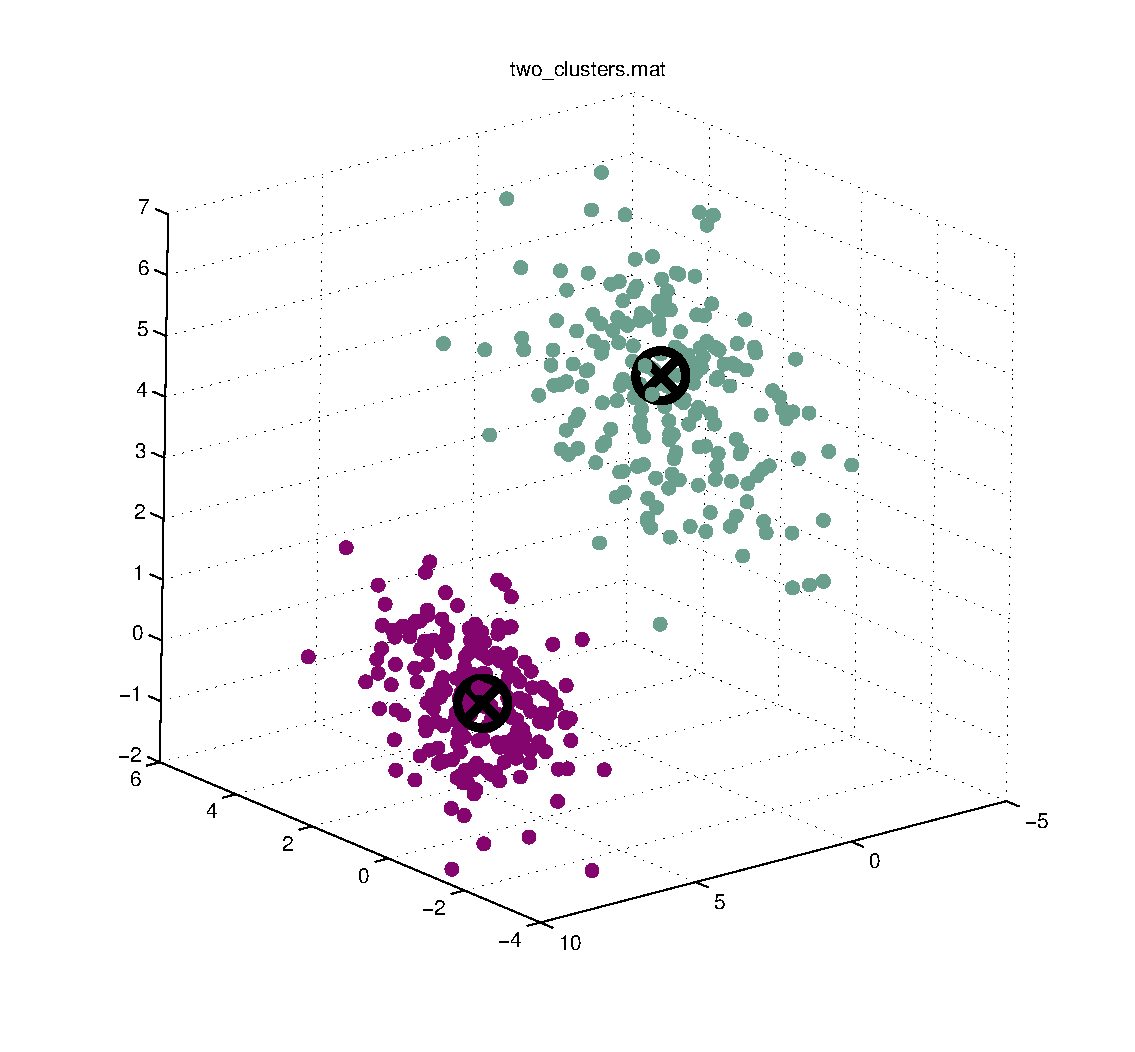
\includegraphics[width=0.8\linewidth]{./figures/clusters.eps}
\caption{Mean Shift Clustering Result}
\label{fig:twoclusters}
\end{center}
\end{figure}


%Given $n$ data points
%$\bf{x_i}$,$i=1,...,n$ in the $d$-dimensional space $R^d$, a kernel density estimate of the
%probability of $x$ is defined as follows:
%\begin{equation}
%\hat p(\bf{x})=\frac{1}{n}\sum_{i=1}^{n}K_{H}(\bf{x}-\bf{x_i})
%\end{equation}
%Here, $K_{H}(\bf{x}-\bf{x_i})$ is a kernel centered at $\bf{x_i}$ with bandwidth $H$.
%To think about this kernel, you can imagine using an isotropic Gaussian centered at $\bf{x_0}$
%with covariance $\Sigma = \sigma I$.

\subsection{Optimizations}
Unfortunately, the Mean Shift algorithm you just implemented is too slow to
be realized for image segmentation.  We will therefore incorporate several
speedups into our implementation. 
\subsubsection{MATLAB vectorization (avoid loops!)}
First of all, you will definitely want to exploit MATLAB's ability to handle matrix
operations efficiently.  For example, if you want to find all data points with label equal
to $1$ and compute their mean, write the following:
\begin{verbatim}
currdata = data(:,labels == 1);
currmean = mean(currdata,2);
\end{verbatim}

You will also be computing Euclidean distances from some $\bf{x}$ to all of your data
very often, and it is crucial that you avoid writing \verb+for+ loops and computing distances
one by one.  We are providing you with a MATLAB function \verb+ml_distSqr+ that given two matrices
of points (where points are the columns in the matrices) as input, will return a matrix of 
squared Euclidean distances between each of the elements in the input.

\subsubsection{Basin and Trajectory of Attraction}

The first non-MATLAB specific speedup will be to associate each data point that is at a 
distance $\leq r$ from the peak with the cluster denoted by that peak. This
speedup is known as basin of attraction and is based on the intuition
that points that are within one window size distance from the peak
will with high probability converge to that peak. \\
\phantom e \\
The second speedup is based on a similar principle, where points that are
within a distance of $\frac{r}{c}$ of the search path are associated with the converged 
peak, where $c$ is some constant value.
Incorporate the above speedups into your Mean Shift implementation
by modifying your implementation from before. The resulting modified function 
should have the following prototypes:
\begin{verbatim}
function [labels, peaks] = meanshift_opt(data,r,c)
function [peak, cpts] = findpeak_opt(data,idx,r,c)
\end{verbatim}
where \verb+cpts+ is a $n$ dimensional boolean vector storing a $1$ for each point that is 
within a distance of $\frac{r}{c}$ from the trajectory or within $r$ from the final peak,
0 otherwise.  Your implementation of \verb+meanshift_opt+ should produce the same result on
\verb+two_clusters.mat+ with $r=2$ and $c=4$ as \verb+meanshift+ (the two clusters will 
start to mix if you let $c=.5$).  You might want to generate some data using \verb+generatedata+
and try to cluster it.  You will have the ground truth labels and can see how well your
algorithm is doing. An example of such a clustering can be seen in Figure \ref{fig:pointcloud}.


\subsection{Image Segmentation}
In this section you will build upon your optimized Mean Shift implementation to perform 
image segmentation. To do so, implement the function
\begin{verbatim}
function [segmIm,peakIm] = segment_meanshift(I,r,c)
\end{verbatim}
In this function, $I$ is a color input image, $r$ is the radius used for our window, and
$c$ is the trajectory of attraction parameter.  \verb+segIm+ is an image created by reshaping
the \verb+labels+ into the size of the input image.  \verb+peakIm+ is an image the same
dimensions as $I$, but with each pixel colored by the RGB value of that pixel's associated
peak.  This function is
constructed by reshaping the image into RGB vectors, converting them to Luv color-space
representation, and then clustering
the resulting color data using the optimized Mean Shift implemented earlier.  Mean Shift clusters 
using the Euclidean distance
metrics, and since Euclidean distance in RGB
space does not correlate well to the perceived change in color we will use Luv color space.
\\
In \verb+segment_meanshift+, convert to Luv color space by using the provided MATLAB 
function \verb+rgb2luv+. Then convert the resulting cluster centers back to RGB using the function \verb+luv2rgb+.

\subsection{Results}

\begin{figure}
\begin{center}
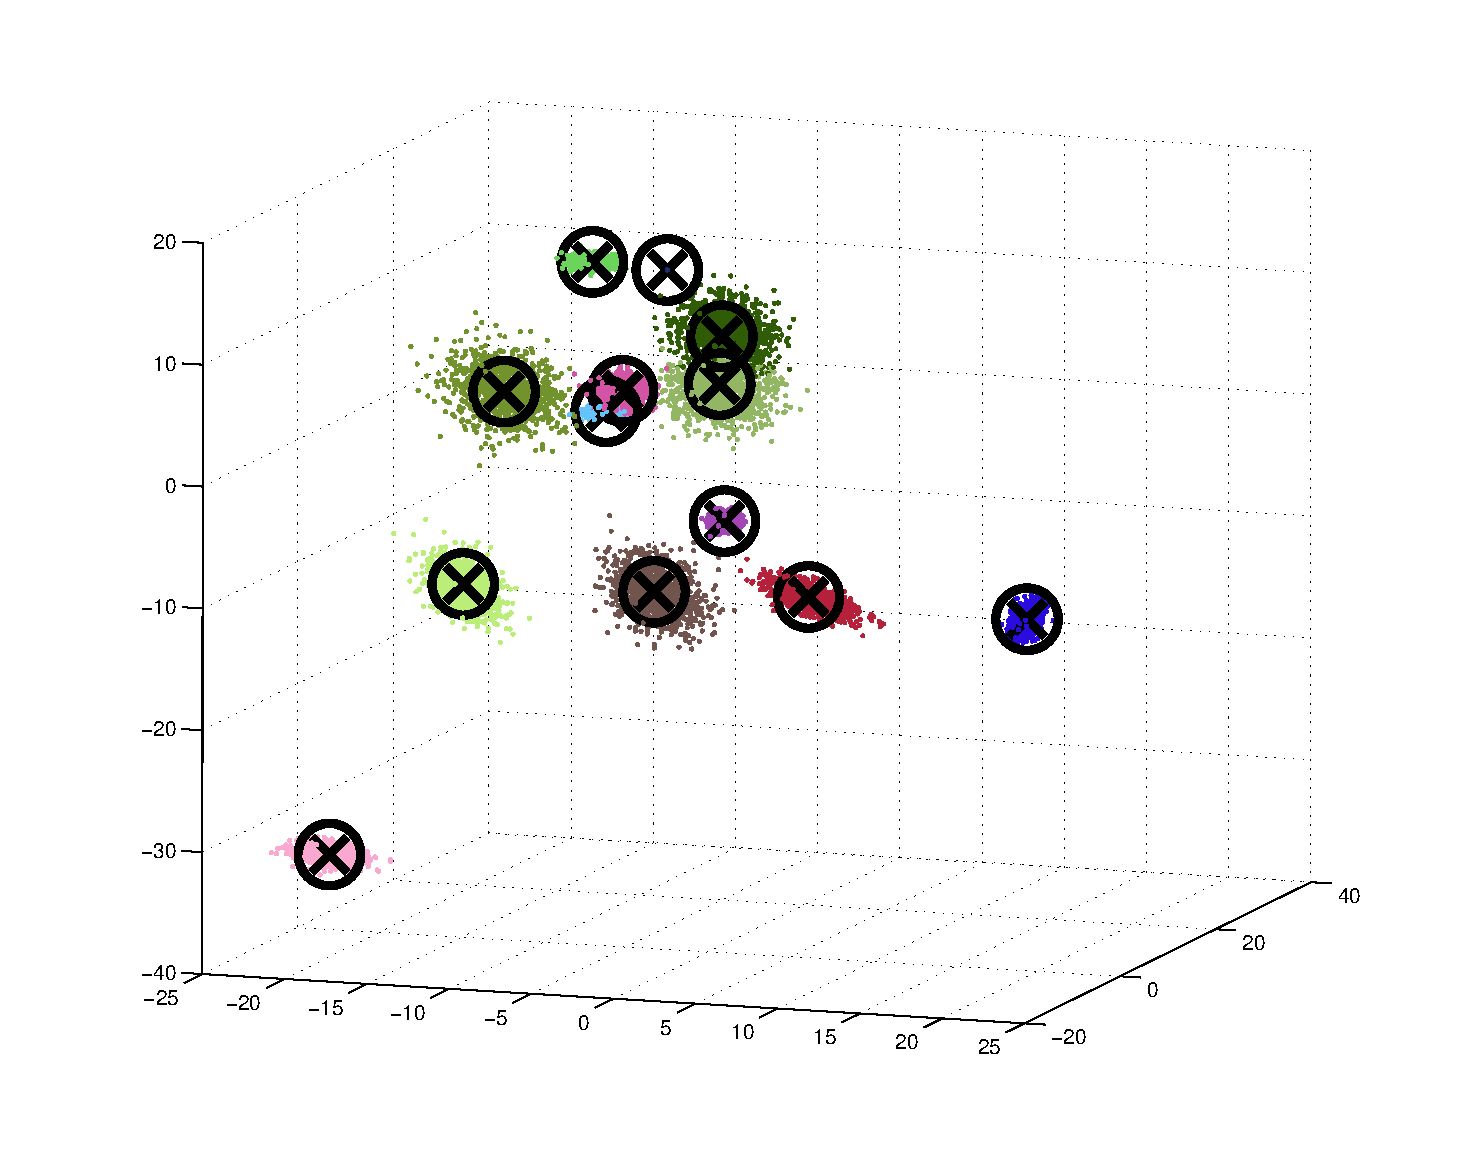
\includegraphics[width=0.8\linewidth]{./figures/more_clusters.eps}
\caption{Mean Shift Segmentation of Point Cloud generated from generatedata function.}
\label{fig:pointcloud}
\end{center}
\end{figure}

First, you will need to cluster the 3D point clouds found in the files \verb+testdata1.mat+,
\verb+testdata2.mat+, and \verb+testdata3.mat+.  You will need to somehow choose a good value
for $r$ and you should use $c=4$.  Produce three result files \verb+results1.mat+, \verb+results2.mat+, and \verb+results3.mat+ such that each file loads the variables \verb+labels+ and 
\verb+peaks+ (the output of \verb+meanshift_opt+).

\begin{figure}
\begin{center}
\includegraphics[width=\linewidth]{./figures/image_starfish2.EPS}
\caption{Mean Shift Clustering Result on Starfish Image. a) label image; b) peak image. This result is generated with $r=20$ and $c=1$.}
\label{fig:starfish}
\end{center}
\end{figure}
You will also have to submit some results on real images.
Note that Mean Shift is still computationally expensive, even with these optimizations.
Furthermore, the computational time depends on the parameters $r$ and $c$. 
For example, with $r= 20, c = 1$, the starfish image in Figure \ref{fig:starfish} took 3 seconds to to segment; and it took 60 seconds to segment if $r= 10, c = 2$. In general, Mean Shift will take longer if $r$ is small and $c$ is big.
In this case, Mean Shift will generate lot of segments which might not be what we want. You will need to play around with different values of $r$ and $c$. With relatively big $r$ and small $c$, your algorithm should not take more  than a few minutes to run. If it does, you are doing something wrong, or you need to stop using punchcard-based computers.


Segment the four \verb+.png+ images (hat,man,star,sheep) using your image segmentation
algorithm.  Experiment with different values of $r$ and $c$ so that you
are able to segment these four images.  Consider $r \in \{5,10,20\}$ and $c \in \{1,2,4\}$.
What effect do $c$ and $r$ have on the run time of your algorithm?  How about the visual
quality of the peaks image?  (You might want to down sample these images when debugging)


%\section{Theory: 30 Points}
%
%1a.) Consider the probabilistic formulation of the problem of fitting a line to a collection 
%of noisy points.  In this formulation, the optimal line parameters are obtained from the
%maximum likelihood estimate.  We also know that the least squares line parameters are the
%same as the maximum likelihood line parameters under the Gaussian noise assumption.
%If we assume that the noise comes from a non-Gaussian distribution, will the maximum likelihood
%solution be equal to the linear least squares solution?  If so, then prove it; otherwise come up with
%an error distribution and its corresponding likelihood where the maximum isn't also the linear least squares solution.
%\\
%\phantom e
%\\
%1b.)Quite often, a problem is that data contains outliers that
%do not come from the same distribution as the remaining points.  These outliers
%can drastically skew our estimates.  What are the
%two algorithms described in class that handle outliers in the estimation process and how do they differ?
%In addition, come up with three standard problems in computer vision where robust fitting techniques can 
%be very useful and what causes the outliers in each problem.
%\\
%\phantom e
%\\
%2.) Assume we have a sequence of $k$ 2D measurements $(x_i,y_i)$ that are obtained from the model
%\begin{eqnarray}
%\left[ \begin{array}{cc}
%x \\
%y \end{array} \right] =
%\left[ \begin{array}{cc}
%u \\
%v \end{array} \right]
%+
%\alpha\left[ \begin{array}{cc}
%a \\
%b \end{array} \right]
%\end{eqnarray}
%where $\alpha \sim N(0,\sigma)$, $au+bv+c=0$ and $a^2+b^2=1$.  In other words, points are generated from a line with
%Gaussian noise perpendicular to the line.
%Under this model, the likelihood of the data $P(D|a,b,c)$ and
%the log likelihood $l(a,b,c)=ln[P(D|a,b,c)]$ are:
%\begin{eqnarray}
%P(D|a,b,c)=\prod_i^k P(x_i,y_i|a,b,c)\\
%l(a,b,c)= -\frac{1}{2\sigma^2}\sum_i^k(ax_i+by_i+c)^2
%\end{eqnarray}
%One can derive the eigenvalue problem
%\begin{eqnarray}
%\left[ \begin{array}{cc}
%\overline{x^2}-\overline{x}\phantom !\overline{x}  & \overline{xy}-\overline{x}\phantom !\overline{y}\\
%\overline{xy}-\overline{x}\phantom !\overline{y} & \overline{y^2}-\overline{y}\phantom !\overline{y}
%\end{array} \right]
%\left[ \begin{array}{c}
%a\\
%b
%\end{array} \right]
%=
%\mu \left[ \begin{array}{c}
%a\\
%b
%\end{array} \right]
%\end{eqnarray}
%from the generative model.  This
%is a relatively simple exercise -- maximum likelihood and
%a little manipulation will do it.  In this problem you are asked to generalize this 2D
%problem to an $n$-D problem (we are dealing with a hyperplane now) where the model is
%$\bf{x} = \bf{u} + \alpha \bf{a}$, $\alpha \sim N(0,\sigma)$, $c+\bf a^T\bf u =0$, and $\bf{a}^T\bf{a}=1$.
%Come up with the $n$-D analog of the log likelihood, set up a constrained optimization problem using lagrange
%multipliers, and derive the form of the corresponding eigenvalue problem.
%\\
%\phantom e
%\\
%3.) Consider the dataset made up of points in Figure \ref{fig:circles}.  How well would you
%expect the following clustering techniques to work on this data set: K-means, Mean Shift, 
%agglomerative clustering, EM for Mixture of Gaussians, and Normalized Cuts?  Which single 
%algorithm would you expect to have the best performance and which algorithms would never be able
%to successfully segment this data set? (Answer in no more than 4-5 sentences)
%\begin{figure}
%\begin{center}
%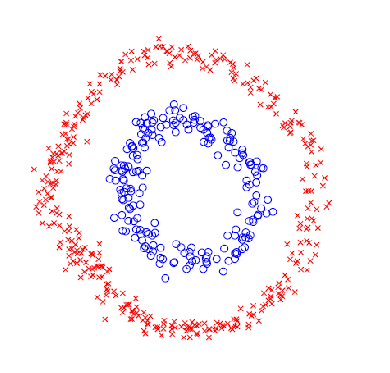
\includegraphics{./figures/circles.eps}
%\caption{Data set made up of two concentric noisy circles.}
%\label{fig:circles}
%\end{center}
%\end{figure}

\section{Segmentation for objects of interest (30 points)}
In many computer vision applications, you might only be interested in a specific class(es) of objects (e.g. horses, faces). Therefore, your image segmentation algorithm needs to be tuned to work for that specific class. In this part of the homework, you will have to provide segmentation results for a set of provided images. 

On the course web page, you can download the dataset that we are going to use for this homework. This dataset consists of 40 images; each image contains a single horse which is considered as the foreground object.
Figure~\ref{fig:figure} displays some of these images. You will soon figure out that using your Mean Shift implementation with color features is not good enough for these images. 

Your task is to extend your current Mean Shift implementation to achieve reasonably good results for the provided images. There are many ways you can extend your implementation, here are some:
\begin{itemize}
	\item Using different features such as color, edges, contours, texture, steerable filters, pixel locations, etc. To achieve good results, you might consider combining different types of features.
	\item Adding post-processing steps to your algorithm such as grouping segments, dividing segments, tracing contours.
	\item Adding prior knowledge: shape prior, location prior.
\end{itemize}

Your extension is not limited to the above list. Moreover, you are not restricted to use the Mean Shift segmentation algorithm from the first part. You are free to propose your own or implement another existing image segmentation algorithm. 

\noindent\textsl{Hints:} You should not use too many features. Irrelevant features might hurt the performance of your segmentation algorithm. Redundant features increase computational cost; Mean Shift (or Matlab) might explode if you use too many features. 

Perfect segmentation is extremely hard and we do not expect the results of your segmentation algorithm to be close to the groundtruth.

\begin{figure}
	\centering
		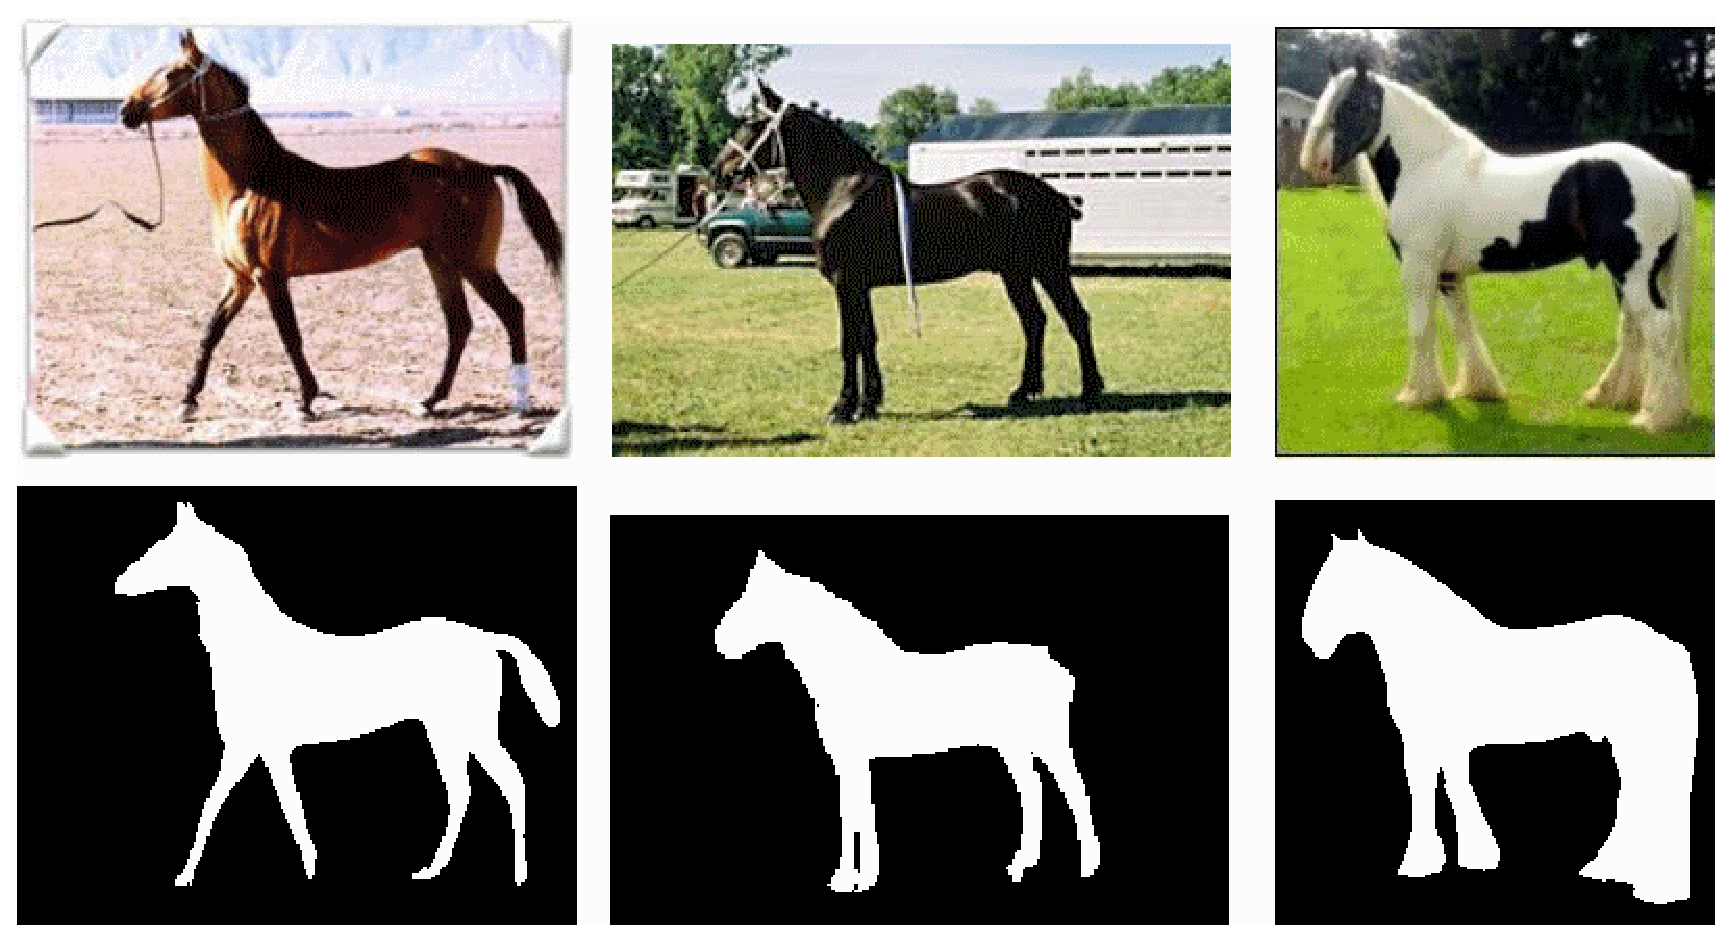
\includegraphics[width=1.00\textwidth]{./figures/figure2.EPS}
	\caption{First row: example of horse images. Second row: the groundtruth foreground masks for the corresponding images in the first row; ideally, the segmentation results should look like the groundtruth masks. However, perfect or close-to-perfect segmentation is SUPER hard. There is no perfect solution to this and we do not expect
things close to the ground truth. }
	\label{fig:figure}
\end{figure}


\subsection{Algorithm design}

%To finish this homework, you can use any material covered in this course. Although you are allowed to
%search reference papers for the state of art techniques, you should be able to finish this homework based
%on the materials covered in class. And you are encouraged to propose your own algorithms. If you do
%choose to implement an existing algorithm from a paper, please cite it in your write-up.
\vskip 0.25cm
\noindent\textbf{Q1}: List the features used by your algorithm, explain why you think they are suitable for this task.

\vskip 0.25cm
\noindent\textbf{Q2}: 
If you extend the Mean Shift algorithm, briefly explain the extension. If implement a different image segmentation algorithm, briefly describe it. You need to highlight the intuitions/ideas/theories underlying it. Your answer to Q2 should exclude things in the answer of Q1.



\subsection{Implementation}
%\subsection{Datasets}
%In the dataset we provide you, there are labels for all the images. These labels are not perfect, for example
%the boundaries of the labels might not exactly correspond with boundary of objects. They might help
%your algorithm in some way, but you are not required to use these labels.
%For each image there is a corresponding .mat �le that contains a pixel-wise labeling of the image. (Ex-
%ample: image 2 10 s.bmp and annotation 2 10 s GT.mat) Loading the annotation �le will load a variable
%groundtruth into the workspace. groundtruth is an image whose dimensions match the dimensions of the
%original image. The pixels will contain one of the following values 0,1,2,3,4,5. An example annotation is
%shown in Figure 1 \& 2. Tree regions are represented as 1, Grass is represented as 2, Building is represented
%as 3, Cow is represented as 4, and Car is represented as 5. All remaining pixels are labeled as 0.
%
%Q3: If you are using the labels, in what way are you using them? If you are not using them, you do not
%need to answer this question.


%You can use all the images in whatever way you want to tune your algorithm. However, you need to provide a brief
%description of how you are making use of the images in your final write up.

\noindent\textbf{Q3}. Write the following function:

\verb|imSegment(input_image_list, path_to_output_directory)|

Running this function will automatically perform image segmentation on a set of images and output the results to a specified directory. \verb|input_image_list| is a cell array of strings that specify the full path of images that one wants to perform segmentation. 
%We have given you an example stored in \textsl{imglist.mat}. Loading this file, you will have a variable called \textsl{imglist} in the Matlab workspace. 
The other input argument, \verb|path_to_output_directory|, is the output directory to store segmentation results. For each input image, your function needs to generate an output segmentation image. The output image must clearly show the segmentation results. Each segment must be associated with one unique color; different segments must be given different colors. 
%The last row of Figure~\ref{fig:figure} shows some examples of output segmentation images. These images are generated by our simple image segmentation algorithm which is based on Mean Shift on the Luv color space. 
The name of the output file should only differ from the input file by the suffix \textsl{\_seg}. For example, if the input image is \textsl{image-032.png}, the output must be named \textsl{image-032\_seg.png} and placed in the directory  \verb|path_to_output_directory|.


%As a way to visually inspect the results, please save a label file for each
%input image. This output file should be the same format as the groundtruth file we described in Section
%1.2.1. Loading this file will load a variable called seg\_result into the workspace, which contains the
%labels defined the same as in the groundtruth file. Name the output file as: \textsl{*\_seg.mat}, where * stands for
%the original input image filename. For example, if the input image is: \textsl{image099.jpg}, the corresponding
%output file will be: \textsl{image099\_seg.mat}.

If your code requires pre-computed data (e.g. parameters, classifiers) that cannot be conveniently stored in the  code, you can store them in \textsl{.mat} files in the same directory with your code. When called, your function must automatically load any necessary data. 

\noindent\textsl{Hint:} The Matlab command `saveas' and `gcf' are quite handy for automatically saving displayed figures.

\subsection{Experiments and tuning}

\noindent\textbf{Q4}. Run your algorithm on the images listed in \textsl{{\bf data/horses/}}, and submit the segmentation results together with your code.  The segmentation images should be placed in \textsl{{\bf results/horses/}}

\vskip 0.25cm
\noindent\textbf{Q5}. As with most computer vision applications, your implementation might not work right away. You are expected to spend a substantially amount of time tuning your function (e.g. size of filters, threshold). To answer this question, you will have to describe how you tune your algorithm.

You are free to used all the images for tuning. You can also use the foreground masks that come with the homework (the second row of Figure~\ref{fig:figure} shows some examples of foreground masks). One way to use these foreground masks is to design a quantitative evaluation and use it for automatic tuning. 
However, you are not required to do so. Yon can tune your method by qualitative evaluation. Whatever method you choose, you have to document it when answering this question.


%
%
%Design a procedure to evaluate the results you get. You might want to design it in a way that can emphasize the differences between your algorithm and others, and show why your algorithm is better.



%\noindent\textbf{Q4}: In which way are you using the images that we have provided you to tune your algorithm?
%
%\noindent\textbf{Q5}: Describe briefly the functionality of your evaluation methods.


%\subsection{Discussion (30 points)}
%Based on the evaluation section, briefly discuss how your algorithm is performing by answering the following questions.
%
%Q6: When you were designing the algorithm, what did you expect for the performance, and what part of
%your hypothesis were proved correct by the results?
%
%Q7: More importantly, if there is any, which part of your hypothesis were proved wrong, and how you
%interpret that? Can you give several examples?


\subsection{Face segmentation challenge (20 bonus points)}
%Many face detector algorithms only provide box output at face positions. It mak
Suppose we are interested in detecting the outer contours of the faces. One idea is to combine the output of a face detector and the an image segmentation algorithm. Given an image, the first step is to run a face detector to find the rectangle region that roughly correspond to the face location. Because the output of the face detector is usually smaller than the face, we enlarge the face detector output so that the enlarged box covers the whole face. The second step is to run an image segmentation algorithm on the enlarged face detector region. The third step is to use the segmented image to find the face contours. 

For this part of the homework, you will have a chance to experiment with this idea and gain some bonus points. The first step of this algorithm has been done for you; the enlarged face detector output regions have been provided as images in the directory \textsl{{\bf data/faces/}}. Your task is to achieve good segmentation results on these images.
We are mostly interested in the face. Here, beard is considered a part of the face but head hairs, neck, and shoulders are not. You do not need to do  the third step. 


\vskip 0.25cm
\noindent\textbf{Q6}. Describe what you did and generate results for the images in \textsl{{\bf data/faces}}. Place the result files in the directory \textsl{{\bf results/faces/}}.


\subsection{Hints}
\begin{itemize}\denselist
	\item Perfect foreground segmentation is NOT required. In fact, it is an extremely hard problem. We are only looking for implementations that provide sensible segmentation results. However, part of your grade for this homework will reflect the relative performance of your algorithm. 
	\item Computational time is not the primary consideration in this homework. However, it should be fast enough
for you to carry out repeatable experiments so that you have time to tune the program. Try to start or tune your algorithm with smaller subset of images first. 
\item Avoid loops in Matlab, practice more with vectorization techniques. 
\item The deadline for this homework is right before the grade due date. Therefore, we will not grant any extension.  Your segmentation algorithm might take several minutes to segment one image. You will need to start the homework early so that you have time to generate the results for 40 horse images. 
\end{itemize}
%We have provided you some facial images 
%
%
%
%We would like to improve the detection qualify by combining the face detector output and the image segmentation. 
%
%
%
%does not really snap to the edges of the faces. 
%
%have implement a reasonably reliable face detector. However, 



\section{Submission}
\begin{itemize}\denselist
\item All source files and any \textbf{\textsl{.mat}} files your functions require. Comments are greatly appreciated. 
%Code for all the functions in the assignment. You should also submit any 
%auxiliary code written to support these functions (Helper functions are OK!).
%And {\em do not} submit the image or annotation data files back to us!  Note
%that in this assignment we have not told you what the function prototypes
%should look like; part of this assignment is to figure this out!
\item \verb+results1.mat+, \verb+results2.mat+, and \verb+results3.mat+ 
\item An image of labels and an image of peaks for each of the four \verb+.png+ images for a total of
$8$ resulting images.  Call the images \verb+sheep_labels.png+, \verb+sheep_peaks.png+, 
\verb+hat_peaks.png+, etc.

\item A file \textbf{\textsl{writeup.xxx}}, where \textbf{\textsl{xxx}} is the extension of the writeup file. The only acceptable file formats are \textsl{pdf, doc}, and \textsl{txt}. This file should contains the answers to all the questions and anything you want us to know about your algorithm. 
%\item All source files and any \textbf{\textsl{.mat}} files your functions require. Comments are greatly appreciated. 
\item The results of your image segmentation algorithm on the set of provided images. The results should be placed in a directory called \textbf{\textsl{results/horses/}} and \textbf{\textsl{results/faces/}}. Furthermore, make sure that this directory ONLY contain the results that we asked; no extra junk please. If you think your algorithm is impressive and you would like to show us other results (e.g. for different types of images, using alternative parameters), please put them in a separate directory called \textbf{\textsl{results/extra/}}. If you do include extra results, please document them in the write-up.
\item DO NOT put any non-result (segmentation images) that we do not ask for in the \textbf{\textsl{results/horses/}} directory.
\item DO NOT submit the images that we provide.
\item DO NOT include your code in the write-up.
\end{itemize}

\noindent \textbf{\Large References}
\normalsize


The theory behind mean shift clustering is described in the following paper:
\begin{verbatim}
``Mean shift: A robust approach toward feature space analysis'' by D. Comaniciu and 
P. Meer, IEEE Trans. Pattern Analysis and Machine Intelligence 24, 2002, 603-619.
\end{verbatim}

Note that there are some errors in the equations and you should look at the 
\verb+meanshift_errata.pdf+ document.  You will not need to understand all of the 
mathematical details of this paper as specifics
of the algorithm that you will be implementing are outlined below.  Of interest is section $4$ 
of the paper, which discusses how a suitable feature space can be defined for image segmentation purposes.


\end{document}
